\documentclass[11pt, a4paper, oneside, fontset=none]{ctexbook}
\usepackage{amsmath, amsthm, amssymb, bm, graphicx, hyperref, mathrsfs, enumitem, geometry, listings, xcolor, listings, fontspec, caption, unicode-math}

% 标题、作者、创建日期
\title{{\Huge{\textbf{XXXXXX}}}\\XXXX}
\author{徐鸣飞}
\date{2023年12月27日}

% 设置全局字体
\setmainfont{TeX Gyre Termes}
\setmathfont{TeX Gyre Termes Math}

% 中文默认字体:方正书宋_GBK,粗体为思源宋体半粗体,斜体为方正楷体_GBK
\setCJKmainfont[Path=../../fonts/, BoldFont=SOURCEHANSERIFCN-MEDIUM-6.otf, ItalicFont=FANGZHENGKAITI-GBK-1.ttf]{FANGZHENGSHUSONG-GBK-1.ttf}
% 中文无衬线字体:方正黑体_GBK,粗体为思源黑体中粗体
\setCJKsansfont[Path=../../fonts/, BoldFont=SOURCEHANSANSSC-MEDIUM-2.otf,AutoFakeSlant]{FANGZHENGHEITI-GBK-1.ttf}
% 中文等宽字体:方正仿宋_GBK
\setCJKmonofont[Path=../../fonts/]{FANGZHENGFANGSONG-GBK-1.ttf}
\newCJKfontfamily\songti{FANGZHENGSHUSONG-GBK-1.ttf}[Path=../../fonts/, BoldFont=SOURCEHANSERIFCN-MEDIUM-6.otf,AutoFakeSlant]
\newCJKfontfamily\xbsong{SOURCEHANSERIFCN-MEDIUM-6.otf}[Path=../../fonts/,AutoFakeBold,AutoFakeSlant]
\newCJKfontfamily\dbsong{SOURCEHANSERIFCN-BOLD-2.otf}[Path=../../fonts/,AutoFakeBold,AutoFakeSlant]
\newCJKfontfamily\cusong{SOURCEHANSERIFCN-HEAVY-4.otf}[Path=../../fonts/,AutoFakeBold,AutoFakeSlant]
\newCJKfontfamily\heiti{FANGZHENGHEITI-GBK-1.ttf}[Path=../../fonts/, BoldFont=SOURCEHANSANSSC-MEDIUM-2.otf,AutoFakeSlant]
\newCJKfontfamily\dahei{SOURCEHANSANSSC-MEDIUM-2.otf}[Path=../../fonts/,AutoFakeBold,AutoFakeSlant]
\newCJKfontfamily\cuhei{SOURCEHANSANSSC-BOLD-2.otf}[Path=../../fonts/,AutoFakeBold,AutoFakeSlant]
\newCJKfontfamily\fangsong{FANGZHENGFANGSONG-GBK-1.ttf}[Path=../../fonts/,AutoFakeBold,AutoFakeSlant]
\newCJKfontfamily\kaiti{FANGZHENGKAITI-GBK-1.ttf}[Path=../../fonts/,AutoFakeBold,AutoFakeSlant]
\newCJKfontfamily\kaishu{FANGZHENGKAITI-GBK-1.ttf}[Path=../../fonts/,AutoFakeBold,AutoFakeSlant]

% 设置页面的尺寸和布局。
\geometry{a4paper,scale=0.75}

% 行间距为1.5倍
\linespread{1.5}

% 生成的书签大纲包含章节序号
\hypersetup{
  bookmarksnumbered=true
}

% 定义定理环境
\newtheorem{theorem}{定理}[chapter]
\newtheorem{definition}[theorem]{定义}
\newtheorem{lemma}[theorem]{引理}
\newtheorem{corollary}[theorem]{推论}
\newtheorem{example}[theorem]{例}
\newtheorem{proposition}[theorem]{命题}

% 自定义配置
% 设置全局的 enumerate、itemize 环境项之间的距离
\setlist[enumerate]{itemsep=-1pt, parsep=0pt, leftmargin=20pt, topsep=5pt, partopsep=0pt}
\setlist[itemize]{itemsep=2pt, parsep=0pt, leftmargin=20pt, topsep=5pt, partopsep=0pt}

% 定义新环境
% 定义颜色
\definecolor{commentcolor}{RGB}{182,73,1}
% 定义代码
\lstnewenvironment{java}[1][]{
  \lstset{
    language=Java,
    basicstyle=\ttfamily,
    keywordstyle=\color{blue},
    commentstyle=\color{green!60!black},
    stringstyle=\color{commentcolor},
    showstringspaces=false,
    breaklines=true,
    frame=single,
    flexiblecolumns=true,
    backgroundcolor=\color{gray!5},
    numbers=left,
    numberstyle=\tiny,
    #1
  }
}{}
\lstnewenvironment{plsql}[1][]{
  \lstset{
    language=SQL,
    morekeywords={BEGIN,DECLARE,END,IF,ELSE,ELSIF,LOOP,WHILE,PROCEDURE,FUNCTION},
    basicstyle=\ttfamily,
    keywordstyle=\color{blue},
    commentstyle=\color{green!60!black},
    stringstyle=\color{commentcolor},
    showstringspaces=false,
    breaklines=true,
    frame=single,
    flexiblecolumns=true,
    backgroundcolor=\color{gray!5},
    numbers=left,
    numberstyle=\tiny,
    #1
  }
}{}

% 定义一个名为ignore的新环境,表示不重要的内容。
\newenvironment{ignore}{%
  \color{gray}% 设置字体颜色为灰色
  \ignorespaces% 忽略环境前的空格
  (% 在灰色文本前添加左括号
}{%
  )% 在灰色文本后添加右括号
  \ignorespacesafterend% 忽略环境后的空格
}

% 文章开始
\begin{document}

% 生成标题
\maketitle

% 生成作者的话
\newpage                    %新的一页
\pagenumbering{roman}       %页码以小写罗马数字形式表示
\setcounter{page}{1}        %设置当前页为第一页
\section*{作者的话}

% 生成目录
\newpage                    %新的一页
\pagenumbering{Roman}       %页码以大写罗马数字形式表示
\setcounter{page}{1}        %设置当前页为第一页
\tableofcontents            %生成目录

% 生成内容
\newpage                    %新的一页
\pagenumbering{arabic}      %页码以阿拉伯数字形式表示
\setcounter{page}{1}        %设置当前页为第一页

% 文章内容
\chapter{文本}
\section{未来的智能社会:人工智能与人类共同进步}
在当今飞速发展的科技时代,人工智能(AI)正逐渐渗透到我们生活的方方面面,为社会带来深远的变革。随着科技不断创新,我们正迈入一个智能社会的时代,人与人工智能将更加紧密地协同合作,共同推动社会的进步。

首先,智能技术在医疗领域的应用将为人类健康带来质的飞跃。未来的医疗设备将配备先进的人工智能系统,能够迅速而准确地诊断疾病,提供个性化的治疗方案。同时,机器人手术助手将能够执行高度精密的手术,减少手术风险,提高治疗成功率。这不仅将极大地提高医疗水平,还将使更多人能够享受到高质量的医疗服务。

教育领域也将因人工智能的介入而发生翻天覆地的变化。个性化的智能教育系统将根据学生的学习特点和需求,量身定制最合适的教学内容和方法。学生将通过与智能教育助手的互动,更加深入地理解知识,培养创新思维和解决问题的能力。这将有助于打破传统教育的条条框框,培养更具创造力和适应力的人才。

\begin{ignore}智能城市的建设也是智能社会发展的一个重要方向。通过大数据和人工智能技术,城市能够更高效地管理交通、能源、环境等方面的问题。智能交通系统将实现车辆的智能导航和交通流的优化,减少拥堵和事故的发生。智能能源管理系统将推动城市向可持续发展方向迈进,减少能源浪费,提高能源利用效率。这将使城市更加宜居,提升居民的生活质量。
\end{ignore}

\textbf{常见的人工智能应用:}
\begin{enumerate}
    \item \textbf{智能交通:} 智能驾驶、交通流优化、车辆和行人识别。
    \item \textbf{金融领域:} 风险管理、欺诈检测、智能投资建议。
    \item \textbf{自然语言处理:} 语音识别、机器翻译、情感分析。
    \item \textbf{智能家居:} 智能家电控制、环境监测、智能安防系统。
    \item \textbf{医疗领域:} 个性化医疗诊断和治疗、医疗图像分析、健康监测。个性化医疗诊断和治疗、医疗图像分析、健康监测。个性化医疗诊断和治疗、医疗图像分析、健康监测。个性化医疗诊断和治疗、医疗图像分析、健康监测。
    \item \textbf{教育领域:} 智能教育系统、个性化学习推荐、在线教育平台。智能教育系统、个性化学习推荐、在线教育平台。智能教育系统、个性化学习推荐、在线教育平台。智能教育系统、个性化学习推荐、在线教育平台。
    \item \textbf{制造业:} 智能制造、预测性维护、机器人生产线。
    \item \textbf{游戏领域:} 游戏智能化设计、虚拟角色智能行为。
    \item \textbf{社交媒体:} 推荐系统、内容过滤、用户行为分析。
    \item \textbf{能源管理:} 智能电网、能源消耗优化、可再生能源预测。
\end{enumerate}

然而,随着人工智能技术的广泛应用,也带来了一些新的问题和挑战。其中之一是人工智能对就业市场的影响。一些传统的工作岗位可能会被自动化取代,需要社会共同努力来提供相关的培训和转岗机会,确保人们能够适应新的就业格局。此外,人工智能的发展也涉及到隐私和安全等重要问题,需要建立健全的法律和伦理框架来保障个人和社会的权益。

总的来说,未来的智能社会将是人工智能与人类共同进步的社会。通过合理而负责任的运用人工智能技术,我们能够在医疗、教育、城市管理等方面取得巨大的成就,推动社会朝着更加智能、可持续和公正的方向发展。然而,我们也需要密切关注人工智能发展中可能出现的问题,通过合作和创新,共同应对挑战,确保人工智能为社会带来更多积极的影响。
\chapter{代码}
\section{java}
\begin{java}[caption=Java程序1]
public class HelloWorld {
    public static void main(String[] args) {
        System.out.println("Hello, World!");
        //so???
    }
}
\end{java}
\section{SQL}
\begin{plsql}[caption=PL/SQL程序1]
    DECLARE
    x NUMBER := 10;
    BEGIN
    IF x > 5 THEN
    DBMS_OUTPUT.PUT_LINE('x is greater than 5');
    ELSE
    DBMS_OUTPUT.PUT_LINE('x is not greater than 5');
    END IF;
    END;
    /
\end{plsql}

\chapter{图片}
\section{浮动图片}
\begin{figure}[htbp]
  \center
  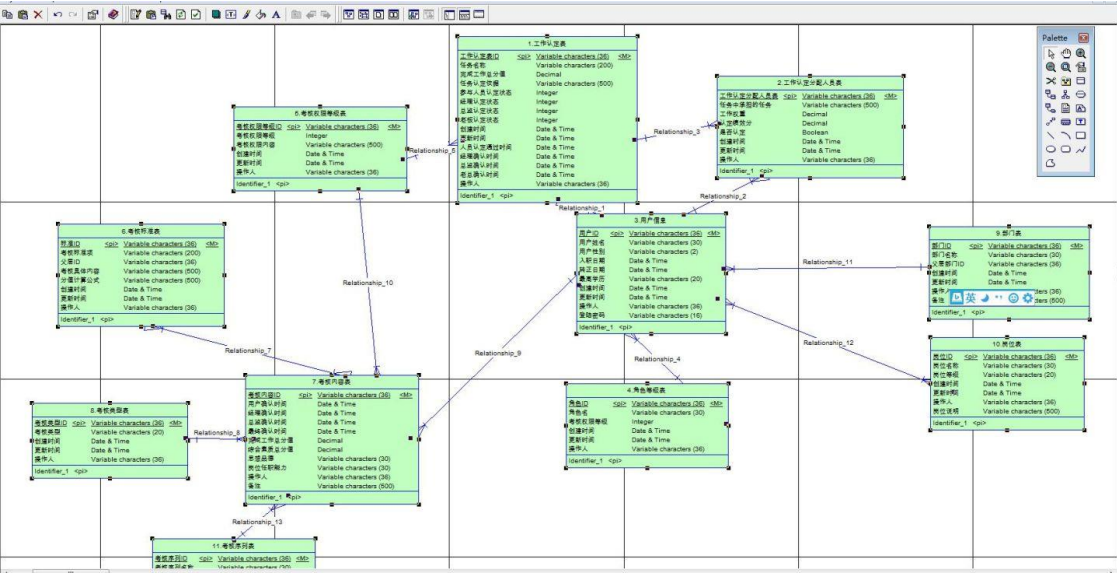
\includegraphics[width=0.5\textwidth]{picture/实体关系数据库示意图.png}
  \caption{实体关系数据库示意图}
  \label{fig:relationDatabase}
\end{figure}
\section{嵌入图片}
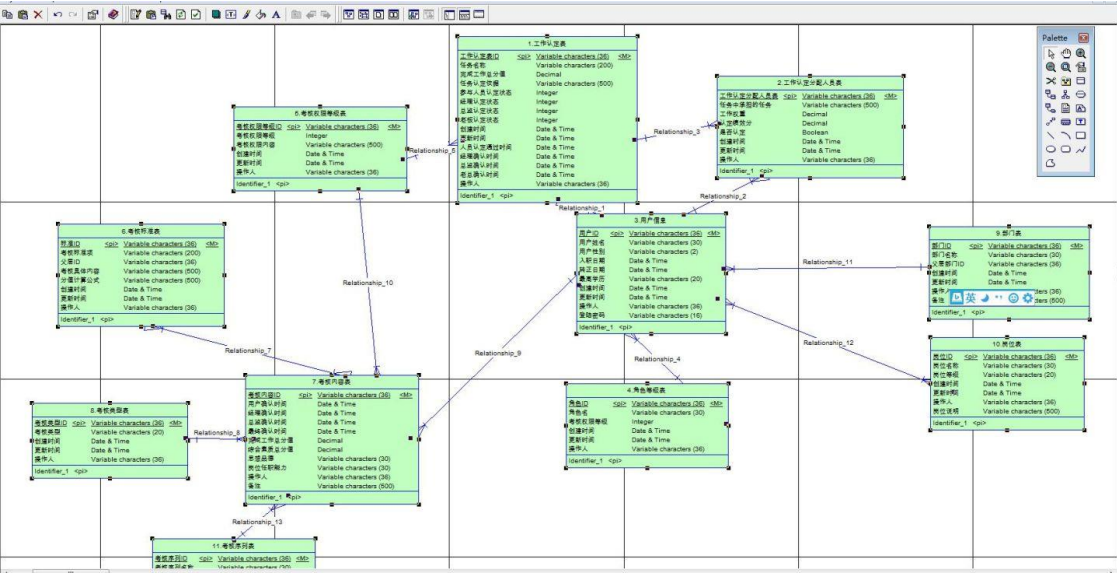
\includegraphics[width=0.5\textwidth]{picture/实体关系数据库示意图.png}
\section{非浮动图片}
\begin{center}
  \begin{minipage}{\textwidth}
    \center
    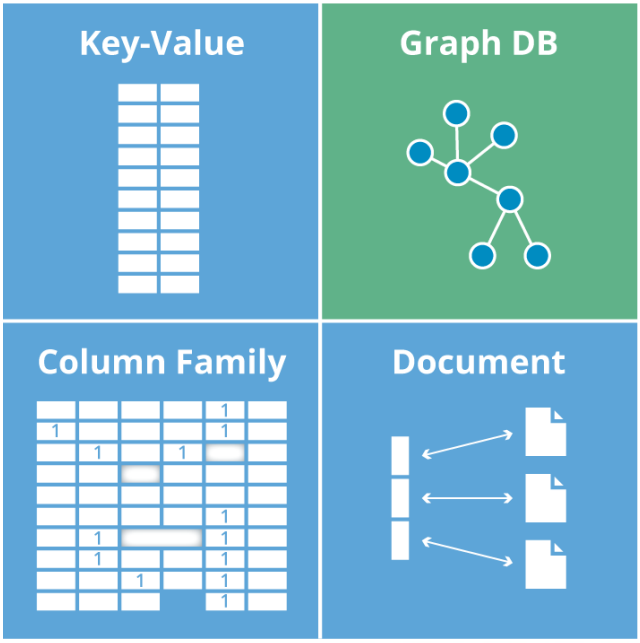
\includegraphics[width=0.5\textwidth]{picture/NoSQL数据库示意图.png}
    \captionsetup{hypcap=false}
    \captionof{figure}{NoSQL数据库示意图}
    \label{fig:NosqlDatabase}
  \end{minipage}
\end{center}

\chapter{字体}
默认字体:方正书宋\_GBK,粗体为思源宋体半粗体,斜体为方正楷体\_GBK

你好abc123\ \textbf{你好abc123}\  \textit{你好abc123}\  
% \textbf{\textit{你好abc123}}

中文无衬线字体:方正黑体\_GBK,粗体为思源黑体中粗体
\textsf{你好abc123}\ \textbf{\textsf{你好abc123}}

中文等宽字体:方正仿宋\_GBK
\texttt{你好abc123}

songti{\songti 你好abc123}

xbsong{\xbsong 你好abc123}

dbsong{\dbsong 你好abc123}

cusong{\cusong 你好abc123}

heiti{\heiti 你好abc123}

dahei{\dahei 你好abc123}

cuhei{\cuhei 你好abc123}

fangsong{\fangsong 你好abc123}

kaiti{\kaiti 你好abc123}

bfserieskaiti{\bfseries\kaiti 你好abc123}
% 文章结束
\end{document}